%% LyX 1.6.5 created this file.  For more info, see http://www.lyx.org/.
%% Do not edit unless you really know what you are doing.
\documentclass[a4paper,english]{IEEEtran}
\usepackage[T1]{fontenc}
\usepackage[latin9]{inputenc}
\usepackage{graphicx}

\makeatletter
%%%%%%%%%%%%%%%%%%%%%%%%%%%%%% User specified LaTeX commands.


\usepackage{babel}

\usepackage[unicode=true, pdfusetitle,
 bookmarks=true,bookmarksnumbered=false,bookmarksopen=false,
 breaklinks=false,pdfborder={0 0 1},backref=false,colorlinks=false]{hyperref}

\makeatother

\makeatother

\usepackage{babel}

\makeatother

\usepackage{babel}

\begin{document}

\date{December 2011}


\author{Alexandre Chappuis, Bastian Marquis and David Klopfenstein @ EPFL.ch}


\title{Implementation of a BGP Route Flap Damping Algorithm for the Bird
Routing Project}
\maketitle
\begin{abstract}
Today's Internet stability strongly relies on the good behavior of
dynamic routing protocols such as BGP (Border Gateway Protocol), that
enables routing between Autonomous Systems. Route flapping is a well-known
and undesirable phenomenon occuring in both commercial and private
networks. In this report, we explain our implementation of the RFC
2439, BGP Route Flap Damping, for one famous Open Source routing software
suite, the Bird Routing Project.

We also present results of an experiment where we compared the number
of BGP updates sent with and without route damping enabled, in a setup
where only one of the bgp router was receiving advertisments for flapping
routes. 
\end{abstract}

\section{Introduction}

The inter-domain routing protocol BGP is still surviving to the gigantic
growth of the Internet that started during the last decade. However,
some widely used applications, such as Skype, still suffer from weaknesses
of that protocol. The main problems are twofolds: Firstly, BGP has
a slow convergence rate, meaning that a change at one location takes
quite some time to be propagated to the other ends of the network.
Secondly, if a node becomes unstable, for example if its connectivity
constantly comes up and down, it will have bad consequences on the
network, both in terms of useless processing at BGP routers and unnecessary
routing traffic. Routes advertised and withdrawn at regular interval
of time are said to be \textit{flapping}.

Many approaches to counter route flapping have been developped in
the late 90's. RFC 2439\cite{rfc2439} standardized one such approach
: it basically blocks updates from flapping routes, and does so until
the routes are deemed stable again. This RFC has been used it extensively
for many years, in both commercial and open source routers.

Although this standard is not recommended anymore\cite{ripe recommendations}
in today's routers, we wanted to implement it for the Bird Routing
Project\cite{bird}, hoping that it will serve as a good basis for
future possible improvements and extensions to this RFC. There exist
many variants of the Route Flap Damping alorithm and the community
has not lost its interest in finding robust mechanisms that could
allow BGP to be more resilient.


\section{Overview}

RFC 2349 seeks to limit the impact of route flapping by {}``damping''
(\textit{i.e.} ignoring packets of) missbehaving routes. The solution
must be able to distinguish flapping routes from good routes, consume
few resources, both in terms of memory usage and process time. The
RFC solves these problems by assigning each route a penalty term.
Whenever this penalty term for a given route reaches a certain threshold,
further advertisements for that route are ignored. This penalty term
varies over time : it is increased when the route becomes unreachable
and decays as long as the route stays stable. As soon as the figure
of merit goes below a \textit{reuse threshold}, the route can be used
again.

The figure of merits decays exponentially over time. Exponential decay
has several advantages : it can be implemented very efficiently using
precomputed \textit{decay arrays}. Also, with exponential decay, the
figure of merit keeps trace of previous instabilities for a fairly
long time : old instabilities become less and less important over
time, while newer ones have more weight.

Network administrators have lots of freedom in choosing the behavior
of the penalty term : they can control the half-life of the penalty
term, its maximum value (thus controlling the maximum time a route
can be suppressed) and both the reuse and cut thresholds.

Here is an example showing how the figure of merit evolves over time
(the illustration comes from \cite{damping-pic}). The route flaps
three times, exceeding the cut threshold only after the third flap.
The route is reused as soon as its penalty term goes below the reuse
limit.

\begin{center}
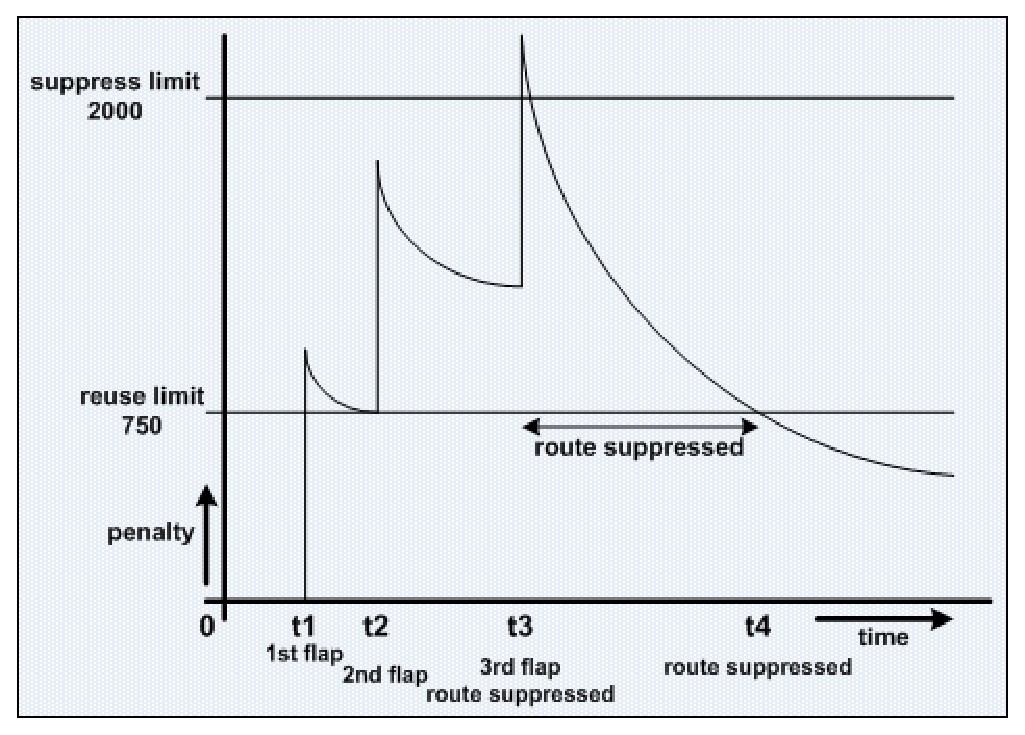
\includegraphics[scale=0.5]{route_damping} 
\par\end{center}

Penalty terms are re-computed at regular time intervals using timers.
Also, every time an update for a route is received, the penalty term
for that route is re-computed.

The RFC proposes several optimizations to decrease processing time,
at the cost of a slightly bigger memory footprint. \textit{E.g. reuse
lists} are used to not have to recompute the figure of merit of all
routes : damped routes with similar penalty terms are grouped together
in a same reuse list. Penalty terms of the routes in a given reuse
list are then re-computed only when necessary.


\section{Implementation}

this part is kind of straightforward -> just explain how we did it
with bird. cite coder's doc + github rep. of code


\subsection{Data structures}


\subsection{Processing withdrawals}


\subsection{Processing route advertisements}


\subsection{Configuration parameters}


\subsection{Timers}


\subsection{Miscellaneous}


\section{Evaluation}

%
\begin{figure}
\caption{Topology used for our simulation}



\end{figure}



\subsection{Overview}

We used a topology of 27 routers in the NSL cluster in order to evaluate
our implementation. This topology consits of 10 Autonomous systems.
Router number 3 with network prefix 10.0.0.3/24 was the the one that
fed the whole network 10.0.0.0/24 with updates coming from one MRT
dump archive (updates.20100401.1729), that we got from the Route Views
project\cite{routeviews}. This archive corresponds to 15 minutes
of real BGP traffic that were sent by 11 BGP routers. The topology
used is represented in figure x.

We ran 3 simulations and recorded every 10 seconds the total number
of updates and withrawals received from all neighbors for all routers.
When route damping was enabled, we also recorded the number of route
dampened at any given time. 
\begin{enumerate}
\item The first simulation was made without route damping and with the official
bird daemon.... 
\item The seconds was made with our bird implementation and default damping
parameters.... 
\item The third was the same as the second, except for the cut\_threshold
parameters that was set to 1000 instead of 1500.... 
\end{enumerate}

\subsection{Evolution of dampened paths}

%
\begin{figure}
\caption{Evolution of dampened paths for Simulation 3}



\end{figure}


it represent time vs. the actual number of dampened routes in AS2
(actually, router 3)

also note that we aggregated results for each AS (for better readability)


\subsection{Number of route updates}

%
\begin{figure}
\caption{Difference of import updates between simulations 1 and 3}



\end{figure}


it's the difference between graph sim1 and graph sim3 -> i.e we have
less updates in SIM3 ! :-)

maybe we can also display one graph with the evolution -> show that
the number is quite huge !! and that's why we show the difference
rather than the two graph on top of each other !


\subsection{Number of withdrawals}

works for sim3, not for sim2 !


\section{Conclusion}

show importance of stability


\section{Future work}

possible extensions

real scale tests


\section{Acknowledgement}
\begin{thebibliography}{6}
\bibitem[1]{rfc2439}The RFC 2439, BGP Route Flap Damping, \href{http://www.ietf.org/rfc/rfc2439.txt}{http://www.ietf.org/rfc/rfc2439.txt}

\bibitem[2]{ripe recommendations} RIPE Recommendations On Route-flap
Damping, \href{http://www.ripe.net/ripe/docs/ripe-378}{http://www.ripe.net/ripe/docs/ripe-378}

\bibitem[3]{bird}Bird Routing Project, \href{http://bird.network.cz}{http://bird.network.cz}

\bibitem[4]{repository}Our publicly available repository, \href{https://github.com/alexchap/Albatros-Project}{https://github.com/alexchap/Albatros-Project}

\bibitem[5]{damping-pic}itcertnotes, \href{www.itcertnotes.com}{http://www.itcertnotes.com}

\bibitem[6]{routeviews}\href{http://routeviews.org}{http://routeviews.org} 
\end{thebibliography}

\end{document}
